\documentclass{article}

\usepackage{graphicx}
\usepackage{amsmath}
\usepackage{amsthm}
\usepackage{float}
\usepackage{hyperref}
\usepackage[margin=1.25in]{geometry}

\theoremstyle{plain}
\newtheorem{definition}{Definition}
\newtheorem{theorem}{Theorem}
\newtheorem{corollary}{Corollary}

\title{Security on Networks}
\date{\today}
\author{Bonny Jain, John Wang, Iris Xu}

\begin{document}

  \maketitle

\section{Simulation Results}

In this section, we provide results from computational simulations of our model. The graphs that we simulate on are created using the Erdos-Renyi mechanism with the number of nodes fixed at $n = 100$. Fixing the number of nodes reduces the number of parameters that can vary.

\subsection{Simulating the Non-Dynamic Model}

To begin, we present results from simulating the non-dynamic model. In this case, each individual chooses his protection $q \in [0,1)$ before the game begins and is not allowed to change his choice as the game proceeds. The individual is not given any idea of what his position in the graph will be, but he does know the probability of edge creation $p$.

  Solving for a mixed strategy Nash Equilibrium in this context is $PPAD$ complete.\footnote{\url{http://www.cs.berkeley.edu/~christos/papers/cacmDGP-2.pdf}} This implies that for all practical purposes, solving for a Nash Equilibrium is computationally intractable, although little is known about the actual complexity of $PPAD$ in relation to $P$ and $NP$.\footnote{\url{http://ieeexplore.ieee.org/xpl/articleDetails.jsp?arnumber=4031362}} 

Because we cannot compute the equilibrium vector of protections $\bar{q}$ where $q_i \in [0,1)$ is player $i$'s choice of protection, we can sweep along a grid of representative values for $\bar{q}$ and examine the game at each one of these values.

Fortunately, this game is symmetric for each player and Acemoglu et al (2013) have shown that under such situations, the Nash Equilibrium for each player is to play the same protection $q$. Therefore it suffices to check setting $q_i = q_j$ for each player $i \neq j$ in our simulations. We shall call $q = q_i$ the protection that each player chooses.

To examine the outcome of a contagion spreading on an Erdos Renyi graph with edge probability $p$, $n = 100$, and protection rate $q$ for each participant, we must be able to compute $\tilde{P}_i(A, q_{-i}, \Phi)$, the probability that the infection reaches $i$ (i.e. the probability that any one of $i$'s neighbors gets infected). However, since computing $\tilde{P}_i$ is NP-hard, we instead use Monte Carlo simulations to approximate $\tilde{P}_i$. We do so in the following manner:

\begin{itemize}
  \item Generate $\kappa$ Erdos Renyi graphs with parameters $G(n, p)$.
  \item For each graph instance and protection value $q$, we run the following for $\gamma$ trials: choose a random node to infect and run the infection to completion.
  \item Compute $\hat{P}$, an estimate of $\tilde{P}_i$ for all $i$, as the total number of infected nodes after $\gamma$ trials divided by the total number of nodes. For $n = 100$, if we let $I_j$ be the number of infected nodes on the $j$th trial, we have:
    \begin{eqnarray}
      \hat{P} = \frac{1}{n \gamma} \sum_{j=1}^{\gamma} I_j
    \end{eqnarray}
  \item Compute the standard deviation of $\hat{P}$ by using standard techniques of computing standard deviations for a sample of random variables from a binomial distribution.
\end{itemize}

In fact, there are provable bounds on how good our Monte Carlo results are for the approximation of $\tilde{P}_i$, given by Karp and Luby (1985) for the All Terminal problem (but can easily be extended to our problem):\footnote{See \url{http://www.sciencedirect.com/science/article/pii/0885064X85900214} for the full proof.}

\begin{theorem}
  To estimate the probability $\tilde{P}_i$ for $i \in V \setminus u$ where $u \in V$ is the source node of the infection to within a multiplicative factor of $1 + \epsilon$ for all $\epsilon \in [0,1]$, it suffices to run the Monte Carlo algorithm for a number of trials given by:
  \begin{eqnarray}
    O \left( \frac{\ln n}{\epsilon^2 \tilde{P}_i} \right)
  \end{eqnarray}
\end{theorem}

\subsection{Simulation Results}

We use the above model to simulate results, with $n = 100$, $\gamma = 250$, and $\kappa = 100$. In order words, we generate $\kappa = 100$ random graphs for each set of Erdos Renyi parameters, then on each graph, we run $\gamma = 250$ distinct infections which each start at a random node. The results are then summarized for different protection rates of $q$.

We begin by presenting the average infection probability $\hat{P}$ when the edge creation probability in Erdos Renyi is very small (we choose $p = 0.005$). Here the Erdos Renyi parameter is $np = 0.5$, which is below the threshold value for the existence of a giant component. Under this regime, the average infection probability $\hat{P}$ is very low for all protection levels (even a protection rate of $q = 0.05$), as seen in the simulation results from figure \ref{avg_prob_np05.fig}.

The intuition behind this is clear. Since $np = 0.5 < 1$, the average size of a component is small, so the amount that the infection can spread is decreased. Thus, even for low protection rates, the infection cannot spread very far.

\begin{figure}[H]
  \centering
  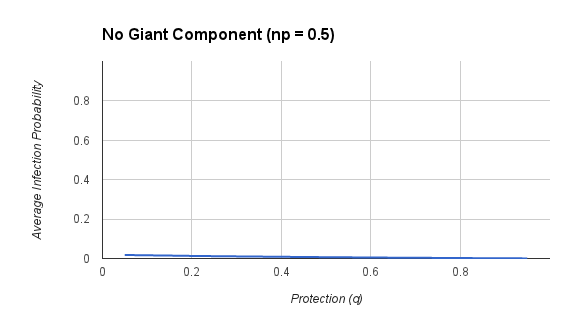
\includegraphics[width=4in]{avg_prob_np05.png}
  \caption{Average Infection Rates with No Giant Component $np = 0.5 < 1$}
  \label{avg_prob_np05.fig}
\end{figure}

When the Erdos Renyi parameter predicts the presence of a giant component, the average infection rate has a strong dependence on the protection rate. We use $np = 5 > 1$ which should produce a giant component with high probability, and simulate the resulting infection probabilities for various values of $q$. Figure \ref{avg_prob_np5.fig} shows the results from our simulations for $np = 5$. For low $q$, the average infection rate is incredibly high. For example, when $q = 0.05$, the average infection rate is $\hat{P} = 0.93$ with a standard deviation of $0.0103$.

As the protection rate increases, the average infection probability decreases almost linearly until about $q = 0.6$. Once $q = 0.6$, the positive externalities start to kick in and the average infection probability drops off more dramatically than the linear trend would predict. This can be attributed to the "network effect", or the extra benefit that everyone obtains from one person increasing their protection. Having higher $q$ will positively impact your neighbors because of the lower probability of you getting infected and thus transmitting to your neighbors. 

\begin{figure}[H]
  \centering
  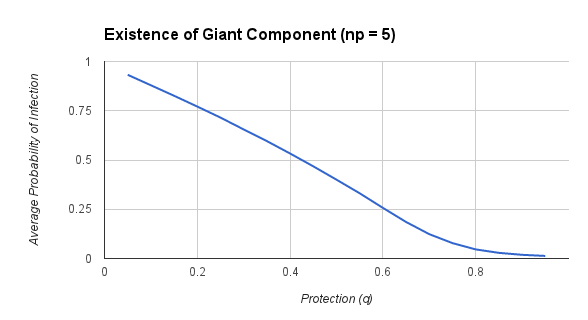
\includegraphics[width=4in]{avg_prob_np5.png}
  \caption{Average Infection Rates with Giant Component $np = 5 > 1$}
  \label{avg_prob_np5.fig}
\end{figure}

However, you must have enough connections in order for this network effect to become substantial. This is why the network effect does not manifest itself when there is no giant component. Figure \ref{network_effects_np5.fig} shows the network effect for different levels of $q$, where network effect $\nu$ is defined as follows:
\begin{eqnarray}
 \nu = 1 - q - \hat{P}
\end{eqnarray}

The network effect starts to increase to something significant by $q = 0.5$, then falls off again after $q = 0.8$. The fall off in the network effect comes from the saturation of protection levels. After a certain point, the marginal benefit of extra protection starts to decrease because of the difficulty of actually spreading the infection.

\begin{figure}[H]
  \centering
  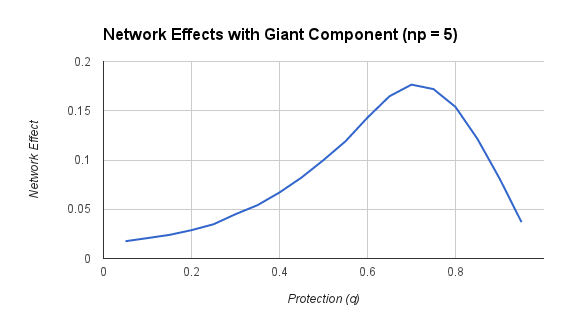
\includegraphics[width=4in]{network_effects_np5.png}
  \caption{Network Effect in a Giant Component ($np = 5$)}
  \label{network_effects_np5.fig}
\end{figure}

\subsection{Computational Intractibility of $\tilde{P}_i$}

Unfortunately, computing $\tilde{P}_i(A, q_{-i}, \Phi)$ in general for a graph which is not a tree is in $\# P$, which is as least as hard as $NP$. This makes computing $\tilde{P}$ computationally intractable.

The reduction can be seen by introducing a known $\# P$ problem called the Two Terminal Problem.

\begin{definition}
  Let us define a graph $G = (V, E)$ with some probability labelling $Pr: E \to [0,1] \cap \mathrm{Q}$. Let $u \in V$ be a source terminal and $v \in V \setminus \{u\}$ be a target terminal. An instance of the \emph{Two Terminal Problem} is to compute $Pr(v | u)$, the probability that there exists a path to node $v$ from node $u$.
\end{definition}

Note that in the Two Terminal Problem, each edge $e \in E$ has some probability of failure $p_e \in [0,1]$ as defined by the function $Pr$.

Showing the difficulty of the computation of $\tilde{P}_i$ in the non-dynamic model is now as simple as showing a reduction of the Two Terminal Problem, since it is $\# P$ complete as shown by Ball (1980).\footnote{\url{http://onlinelibrary.wiley.com/doi/10.1002/net.3230100206/pdf}}

\begin{theorem}
  Computing $\tilde{P}_i(A, q_{-i}, \Phi)$ for all $i \in \{1, \ldots, n\}$ on an Erdos Renyi graph with edge probability $p$ is $\# P$ hard in the non-dynamic model.
\end{theorem}
\begin{proof}
  We shall show that every instance of the Two Terminal Problem is an instance of the Epidemic Probability Problem (what we shall call the problem of computing $\tilde{P}_i$ in our model).

  Suppose we have an instance $\pi_{ttp}$ of the Two Terminal Problem. We can find a solution as follows:
  \begin{itemize}
    \item Create an instance $\pi_{epp}$ of the Epidemic Probability Problem using graph $G$ from $\pi_{ttp}$.
    \item Set the protection rates $q_e \in [0,1)$ for each edge $e \in E$ for the Epidemic Probability Problem as $1 - Pr(e)$, where $Pr(e)$ is the loss probability for edge $e$ in the Two Terminal Problem.
    \item Solve the Epidemic Probability Problem. The probability $\tilde{P}_v$ for a given source of infection $u$ will be the solution to the Two Terminal Problem.
  \end{itemize}

  Thus, we have shown that the Two Terminal Terminal problem can be reduced in polynomial time to the Epidemic Probability Problem, which shows that the Epidemic Probability Problem is at least as hard as the Two Terminal Problem (which is $\# P$ hard).
\end{proof}

The complexity result can be extended to the dynamic case when the protection for each node potentially changes. This means that for both the non-dynamic and the dynamic model, the computation of $\tilde{P}_i$ is computationally intractable.

\begin{corollary}
  Computing $\tilde{P}_i(A, q_{-i}, \Phi)$ for all $i \in \{1, \ldots, n\}$ on an Erdos Renyi graph with edge probability $p$ is $\# P$ hard is the dynamic model with changes in protection in each time step.
\end{corollary}
\begin{proof}
  We can reduce the Two Terminal Problem to the Dynamic Epidemic Probability Problem, where the probabilities are fixed to represent $Pr$ from the Two Terminal Problem. Using the same derivation as before, we can show that the dynamic version of the Epidemic Probability Problem is $\# P$ hard.
\end{proof}

\subsection{Computationally Intractable Problems}

There are a number of related problems which are computationally hard. Actually, most interesting quantities related to the epidemic problem are NP-hard to compute. For example, computing the expected number of infected nodes is NP-hard.

\begin{theorem}
  Computing the expected number of infected nodes on the an epidemic network with protections $q_i$ for $i \in \{1, \ldots, n\}$ is $\# P$ hard.
\end{theorem}
\begin{proof}
  We shall reduce the Epidemic Probability Problem to the Epidemic Expected Infection Problem (the problem of computing the expected number of infected nodes in an epidemic network).

  Suppose we have an instance of the Epidemic Probability Problem. Now select a node $u \in V$ and create a new node $v \not \in V$ which will be attached to the graph. Now, create an edge $e(u,v)$ between $u$ and $v$ and set $v$'s protection to $q = 0$. Now, if $u$ is ever infected, then $v$ will also be infected.

  It is clear that the expected number of infected nodes in this new graph increases by $P_i(u)$, the probability of $u$ becoming infected. Thus, finding the expected number of infected nodes is at least as hard as finding the probability of infection of a node. Thus, we see that the Epidemic Expected Infection Problem is harder than the Epidemic Probability Problem, which is in $\# P$.
\end{proof}

\section{Fast FPTAS for Infection Probabilities}

Although the problem of solving for infection probabilities is $\# P$ hard, it is still possible to approximate the probabilities. In fact, Karger (1999) developed a Fully Polynomial Time Approximation Scheme (FPTAS) for solving the all terminal problem, which can be defined as follows: given a graph $G = (V,E)$ and a probability function on the edges $Pr: E \to [0,1]$ of the probability of any edge failing, find the probability that the entire graph remains connected after edge failures occur with probability $Pr(e)$ for each edge $e \in E$.

An FPTAS is an incredibly strong result, as it means that for any $\epsilon > 0$, one can use the FPTAS to approximate the result to within a factor of $1 + \epsilon$ in time polynomial in the inputs and $\epsilon$. Thus, one can get arbitrarily close to the exact result by using a smaller and smaller $\epsilon$, in exchange for a higher running time.

There exists a naive generalization of Karger's FPTAS to the problem of computing all infection probabilities. In this section, we provide an overview of Karger's FPTAS, it's naive generalization to computing multiple-source multiple-sink infection probabilities (MSMSIP), and finally an asymptotically faster FPTAS than the naive algorithm for MSMSIP.

\subsection{Multiple-Source Multiple-Sink Infection Probabilities}

First we define the problem of computing infection probabilities for multiple sources and multiple sinks.

\begin{definition}
    We will be given a graph $G = (V,E)$ and some function of protections $Q: E \to [0,1)$ which defines the protection $q_v$ inherent for the infection to move down edge $(u,v)$. The \emph{MSMSIP problem} is to find the probability of infection $P_i(u)$ for each node $i \in V \setminus u$ for all possible starting nodes $u \in V$.
  \end{definition}

  Since we have shown the single-source single-sink infection probability problem to be $\# P$, it must be the case that MSMSIP is also $\# P$ because solving the MSMSIP implies that you have also solved the singular problem.

\subsection{Summary of Karger's FPTAS for the All Terminal Problem}

Karger solves the all terminal problem using a combination of a minimum cut finding algorithm and the Monte Carlo scheme. If $\tilde{P}_i$ is large, then it is sufficient to use the Monte Carlo algorithm because of the time bound of $O(\log n / (\epsilon^2 \tilde{P}))$. However, when $\tilde{P}$ is small and arbitrarily close to zero, the Monte Carlo simulation requires a prohibitive number of trials. Therefore, Karger develops another polynomial time algorithm which can be used when $\tilde{P} < 1/n^4$. When this is the case, we can find cuts that are small enough, and these cuts will provide an easy way to estimate the probability of failure.

To make this argument more rigorous, we shall develop the theory more formally. Notice that graphs become disconnected exactly when all the edges in a cut fail. Thus, it is clear that if each edge $i$ in a cut fails with probability $q_i$, then the cut will fail with probability $\prod_i q_i$. Karger proves the following useful lemma.

\begin{lemma}
  Suppose $c$ is the weight of the minimum cut and an $\alpha$-minimum cut is any cut with weight less than or equal to $\alpha c$, then there are at most $n^{\alpha c}$ $\alpha$-minimum cuts.
\end{lemma}

Karger (1999) also shows that when the probability of the minimum cut failing is small, then we only need to determine the probability that a cut of value close to $c$ fails. The paper proceeds to show that it is sufficient to find the all $\alpha$-minimum cuts, of which there are $O(n^{\alpha c})$ using Karger's Recursive Contraction Algorithm. This produces a set of near minimum cuts, from which we can then compute the loss probability
Now suppose that $c$ is the weight of the minimum cut. Karger proves the fo


\end{document}
